\clearpage
\section{Pileup \label{sec:pileup}}
Due to the high LHC luminosity in the 2011, several proton collisions are taking place simultaneously in one bunch crossing. The number of reconstructed primary vertices per event is shown in Figure \ref{fig:Npv}. The constant change of the luminosity conditions makes a correct simulation in the Monte Carlo samples difficult. We therefore use Figure \ref{fig:Npv} to obtain reweighting factors to equalize the vertex multiplicity in Monte Carlo. The reweighting procedure has been applied for the results shown in Section \ref{sec:impactparameter} to \ref{sec:muonjets}.

\begin{figure}[h!]
\centering
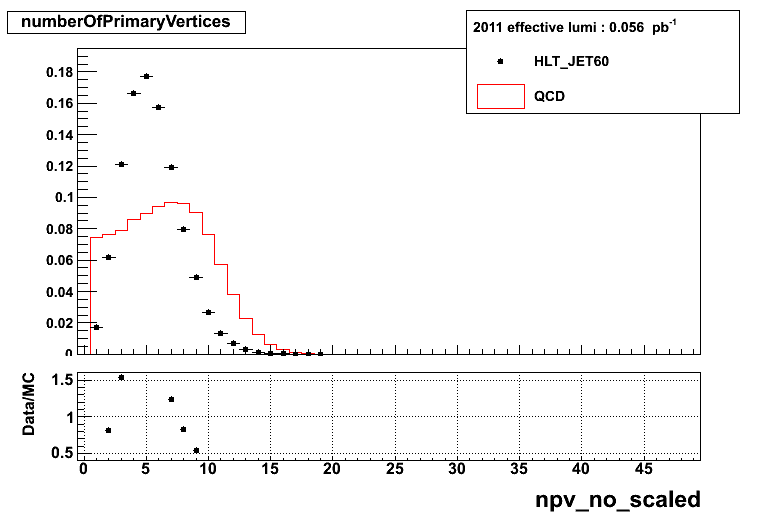
\includegraphics[width=0.49\textwidth]{figures/npv_no_scaled_Linear.png}
\caption{Number of reconstructed primary vertices per event.}
\label{fig:Npv}
\end{figure}

The signal primary vertex is chosen to be the one with the largest sum of track $p_t^2$ which is currently the standard CMS convention. Tracks from pileup vertices can be wrongly associated to a jet from the signal vertex. This effect is visible in Figure \ref{fig:pvNTracks} (left) which shows the number of tracks associated to a jet for three different primary vertex multiplicities. The right plot in Figure \ref{fig:pvNTracks} shows the number of selected tracks. The track selection is clearly rejecting those additional tracks from nearby primary vertices. The most efficient observable to  reject pileup tracks is the distance of the track to the jet axis (compare Section \ref{sec:trackselection}). In the ideal case, tracks from B decays are tangential to the jet axis and therefore have zero distance to the jet axis. Tracks  from pileup events are well separated from the jet axis in longitudinal direction.

\begin{figure}[h!]
\centering
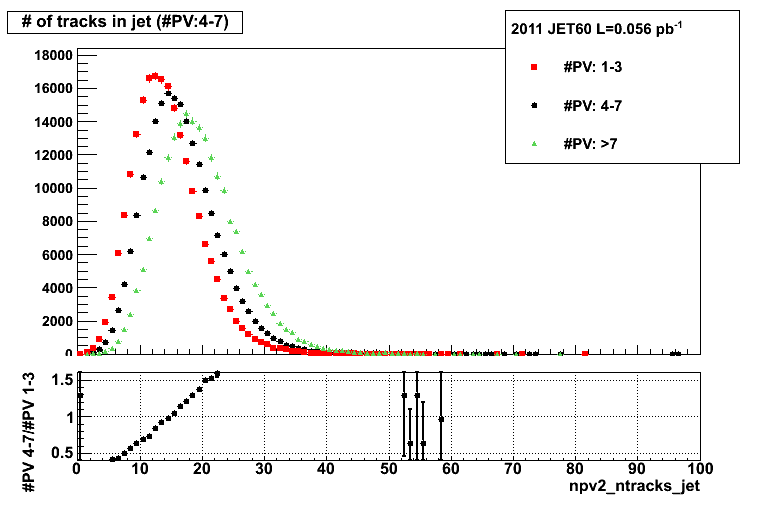
\includegraphics[width=0.42\textwidth]{figures/npv_ntracks_jet_Linear.png}
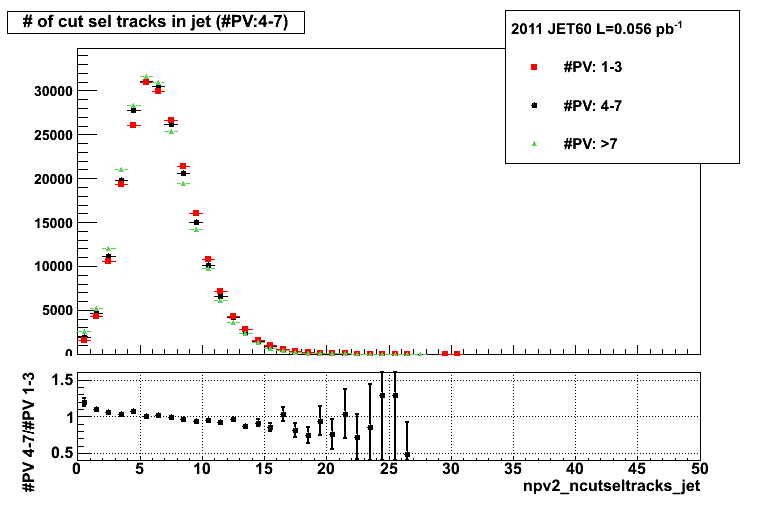
\includegraphics[width=0.42\textwidth]{figures/npv_ncutseltracks_jet_Linear.png}
\caption{Left: number of tracks associated to a jet without any selection cuts. Right: number of tracks associated to a jet passing the selection cuts.}
\label{fig:pvNTracks}
\end{figure}

Some additional validation plots, for three different vertex multiplicities are shown in Figure \ref{fig:pvSVobservables}. The most important observables, such as impact parameter and vertex flight distance seem to be in good agreement among the different pileup multiplicities.  The number of reconstructed secondary vertices per jet for the three pileup cases is shown in Figure \ref{fig:pvSVmult}.




\begin{figure}[h!]
\centering
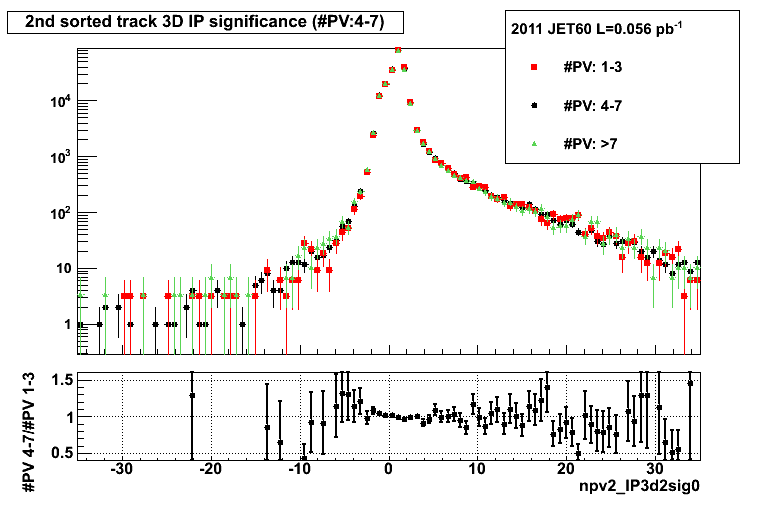
\includegraphics[width=0.32\textwidth]{figures/npv_IP3d2sig0_Log.png}
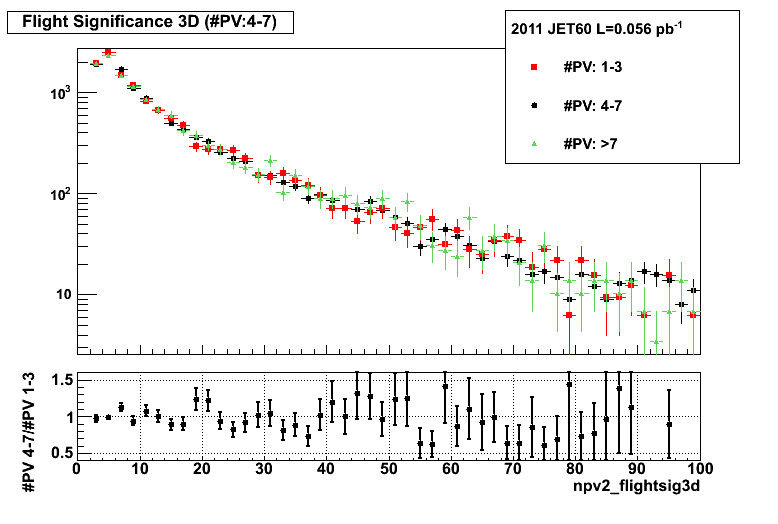
\includegraphics[width=0.32\textwidth]{figures/npv_flightsig3d_Log.png}
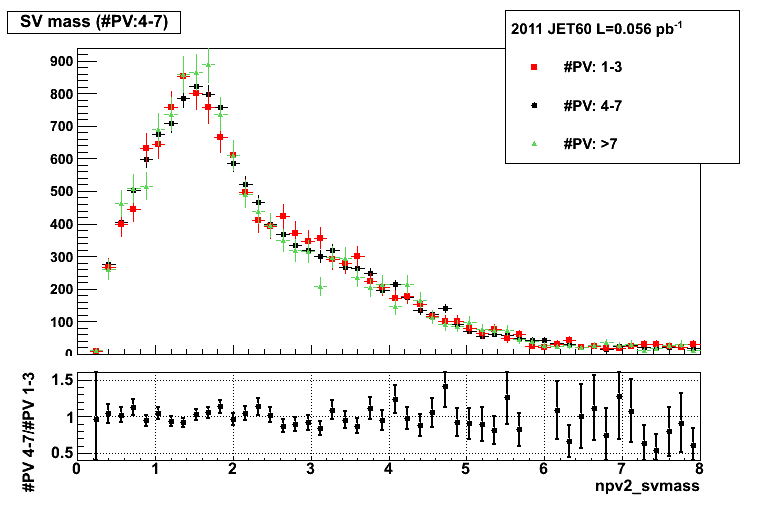
\includegraphics[width=0.32\textwidth]{figures/npv_svmass_Linear.png}
\caption{Left: impact parameter significance of the second track, ordered by IP significance. Middle: secondary vertex flight distance significance. Right: secondary vertex mass. All distributions are split into three different primary vertex multiplicities.}
\label{fig:pvSVobservables}
\end{figure}

\begin{figure}[h!]
\centering
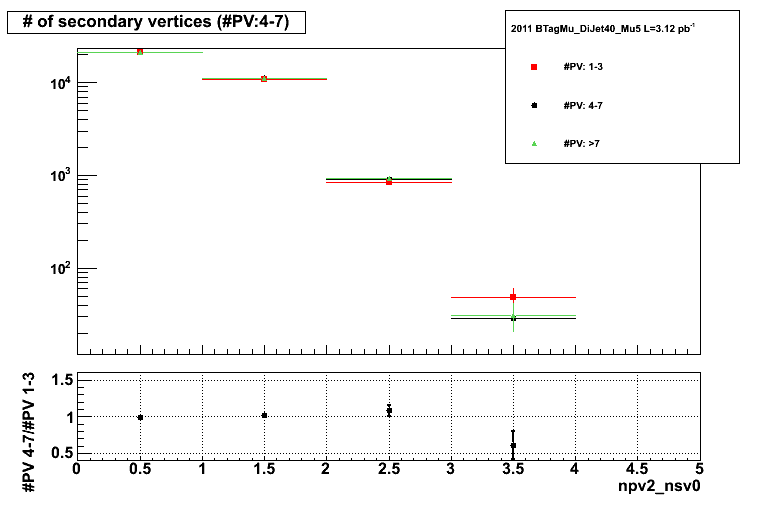
\includegraphics[width=0.42\textwidth]{figures/npv_nsv0_Log.png}
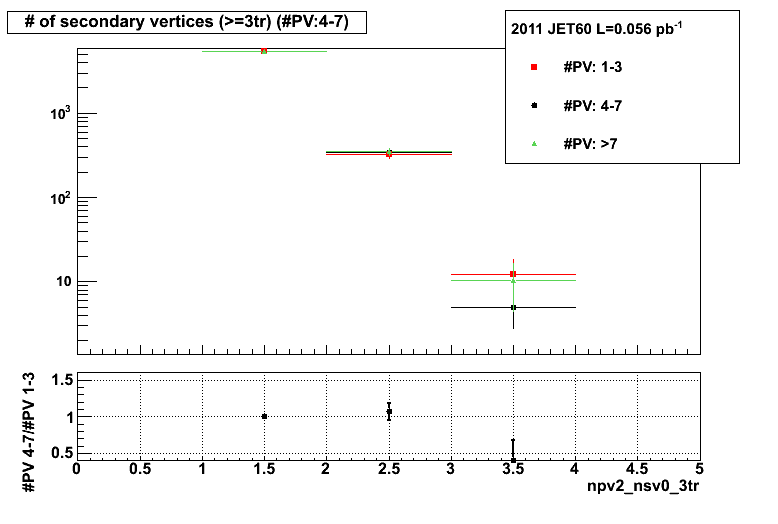
\includegraphics[width=0.42\textwidth]{figures/npv_nsv0_3tr_Log.png}
\caption{Left (right): number of reconstructed secondary vertices with three (two) tracks per jet. The distributions are split into three different primary vertex multiplicities.}
\label{fig:pvSVmult}
\end{figure}


However, Figure \ref{fig:pvNTracks} (right) indicates a slightly reduced track selection efficiency for high pileup multiplicities, because the average number of tracks decreases with more pileup. This results in a reduced b-tagging efficiency in pileup events.
A Monte Carlo based study has been done which shows a clear degradation of the b-tagging performance for events with pileup. This is illustrated in Figure \ref{fig:pileupBTagPerformance} which shows the light flavor mistag efficiency versus b-tagging efficiency for several b-tagging algorithms.

\begin{figure}[h!]
\centering
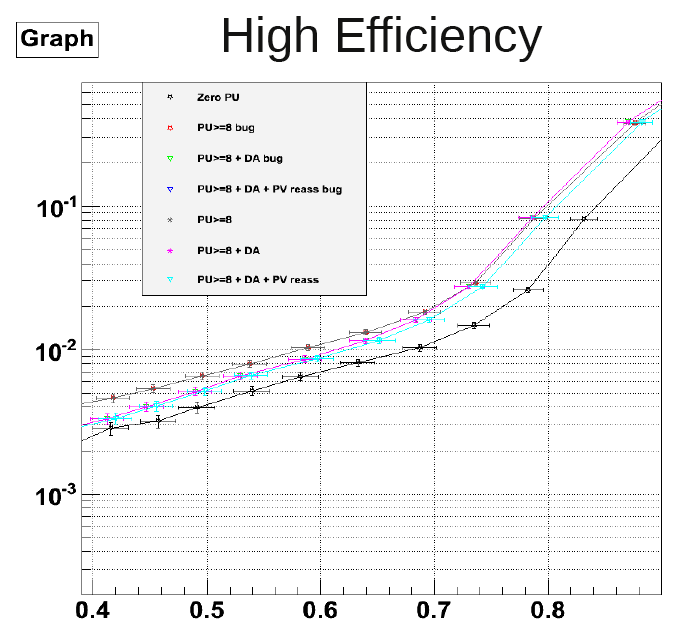
\includegraphics[width=0.32\textwidth]{figures/pileupPerfTCHE.png}
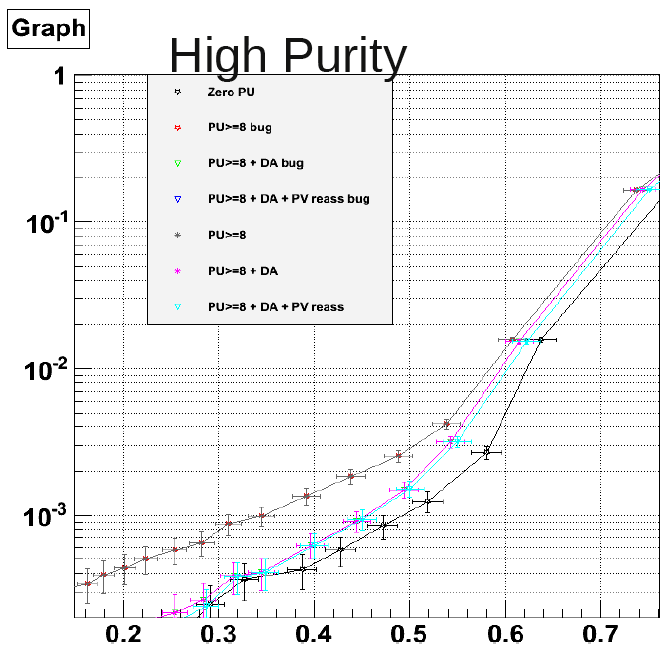
\includegraphics[width=0.32\textwidth]{figures/pileupPerfTCHP.png}
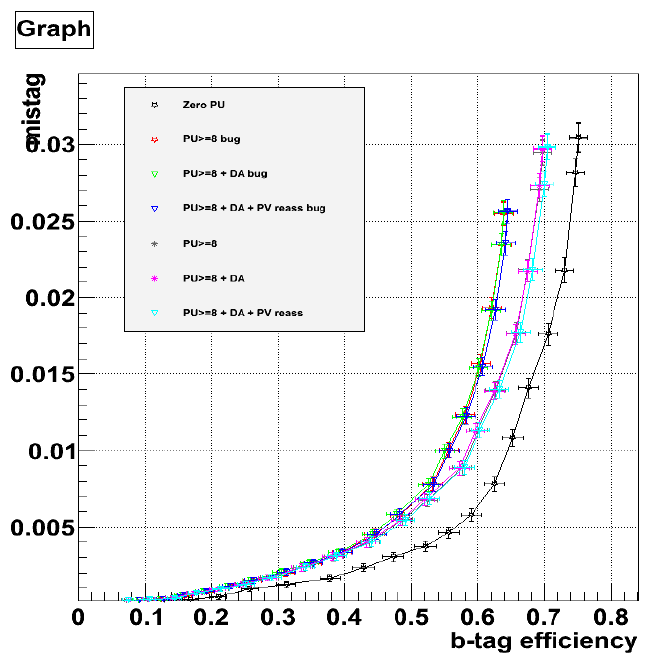
\includegraphics[width=0.32\textwidth]{figures/pileupPerfSSV.png}
\caption{Light flavor mistag efficiency versus b-tagging efficiency for different piluep scenarios. ({\bf FIXME: produce plots properly}). Left: track counting high efficiency algorithm. Middle: track counting high purity algorithm. Right: simple secondary vertex high efficiency algorithm. }
\label{fig:pileupBTagPerformance}
\end{figure}


({\bf FIXME:})    discussion on PV-jet association